\chapter[SCP-107 空龟壳]{
    SCP-107 The Turtle Shell\\
    SCP-107 空龟壳
}

\label{chap:SCP-107}

\begin{figure}[H]
    \centering
    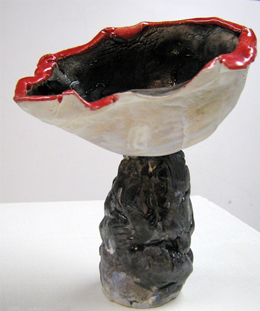
\includegraphics[width=0.5\linewidth]{images/SCP.107.jpg}
    \caption*{非激活状态的SCP-107}
\end{figure}

\bb{项目编号:}SCP-107

\bb{项目等级:}Safe

\bb{特殊收容措施:}只要不接触任何到液体,SCP-107将不会有直接威胁。同时,它被保存在一个位于Site-19中,装在一个有着1m高底座的透明有机玻璃盒子中,存放在一间体积为5立方米的的特别密室中。任何出于研究SCP-107的实验必须在位于6号研究区中的█████████,一块面积为484km\textsuperscript{2}(22km*22km)的专用偏僻区域进行。允许使用一切必要的措施清除在批准的实验之外激活SCP-107的任何人。

接近并搬走此项目需要两(2)名4级人员的许可,而且申请人必须要报告其完整的实验程序。当SCP-107在Site-19进入激活状态时,应由两名D级人员用一辆停在装载区-02的项目运输卡车将其运出。该程序必须追踪任何激活SCP-107的物质,同时能提交改该项目对变化莫测的自然植物方面产生的影响。SCP-107只有在降雨完全停止,同时受感染的畸形植物被清除或者被以日后研究为目的收容之后,才能取回。

\bb{描述:}SCP-107有一个似于一个空的龟壳顶部部分的结构,这个壳是由一种未知源的硬化生物材料所组成。尽管他的外形,包括材料本身,看起来都是一只普通的海龟(\ii{海龟}总科)的龟壳,但是组成成分至今未知。该项目在龟壳部分未接触到液体时完全处于休眠状态;但是在接触到任意一种液体之后,该项目内的液体会被立刻吸收。这些液体被吸收到了哪里是未知的,根据分析,龟壳的内部很少有可见的毛孔。当项目被激活之后,龟壳红色的边缘似乎会开始生长,同时,位于龟壳内部的物质会在空气中凝结中,然后像“雨”一样降落于以该项目为中心最小0.5m,最大10km的范围内。而且,这种现象是可以移动的,运动中的SCP-107会导致这片禁区的影响范围也会随之移动。

实验已证明,SCP-107这一现象持续时间和强度和被龟壳吸收的液体量有关。10ml的水只会导致仅约半个小时的轻度细雨,而装满龟壳四分之三时,造成了持续两天的暴雨。由此现象产生的SCP-107造成的降雨对植物会产生不同的作用,虽然这种影响只在SCP-107作用范围之内的生长的植物上被观察到,收集这些液体并用来浇灌其他的植物未导致异常现象。(见实验日志,附录 107-2)

\hr

\bb{附录 107-1:}SCP-107是被教授M███████ ████████████——一名考古学家所发现,发现地址位于现在的埃塞俄比亚,项目被藏在一位看起来是部落萨满的人的身边。C-14测试显示,这名萨满的骨龄可追溯到公元前18000年。目前已经证实,SCP-107可以抵抗所有损坏,试图从它上面取得样本的行动均已失败告终,因此无法确定该项目的起源日期。基金会在拦截到关于挖掘现场的奇怪天气及植物的异常生长的报告后介入。

\hr

\bb{附录 107-2:} 以下是所有的围绕SCP-107所展开的实验的记录。\dd{对将来的测试协议有合理想法的特工请联系我。}允许使用合理的安全液体进行对SCP-107进行实验,然后记录实验结果(同时请注意,你要对接下来实验会产生的任何结果负全责)。我们需要所有能从这件反常的东西上能获得的数据。更多基于液态SCP的实验也许会有研究价值,但是他们中的大部分由于用来进行实验会显得过于危险,特别在当前的遏制程序下。已经有人建议开展SCP-107涉及到\hyperref[chap:SCP-009]{SCP-009},\hyperref[chap:SCP-447]{SCP-447-2}和\hyperref[chap:SCP-874]{SCP-874}的测试,但是由于实验的高度不稳定性和潜在的危险性而被回绝。——Quentin l███████博士

\bb{加入物:}10ml标准自来水\\
\bb{结果:}测试点周围产生了持续27分钟的小雨,收集到的雨水并未显示出有什么异常。在实验至少两周之后,观测到实验区的草出现了惊人的增长素率,而且这些植物相比起未受影响的地区植物,含有更丰富的叶绿素。\\
\bb{更多研究:}收集了一份雨水的样本,并用来浇灌多种其他不处于测试区的植物。\\
\bb{结果:}没有任何特别的效果被观测到。

\bb{加入物:}55ml标准自来水\\
\bb{结果:}测试区产生持续两天的暴雨,测试区的植物产生了和第一组实验类似的结果。生长在测试区的结实植物被观测到有着非常快的生长速度,而且结出了比对照组植物大得多的果实。之后观测到,在三个月之后,SCP-107的影响变得弱了很多。

\bb{加入物:}4cm\textsuperscript{3}的木块\\
\bb{结果:}没有观测到任何现象。

\bb{加入物:}20颗半径2mm的钢球\\
\bb{结果:}没有观测到任何现象。

\bb{加入物:}10ml人类尿液\\
\bb{结果:}在测试区产生了持续27分钟的中等强度尿液雨。测试区的草开始死亡,所有其他被移栽进测试区的植物开始长出猪笼草状结构,但因发育受阻而无法消化昆虫。\\
\bb{进一步的实验:}20ml人类尿液\\
\bb{结果:}尿雨以稍微强一点的强度在测试区持续了3小时42分。非草本植物比之前长出了更大的,类似猪笼草的捕食结构,而且已经强大到可以捕食小型啮齿动物。

\bb{加入物:}10ml提取自D级非安保人员对象的人类血液\\
\bb{结果:}在下了一场持续27分钟,基因组成与目标D级人员基因相同的人血雨后。在测试区的草在与血接触的时候出现死亡,并且在几分钟内就腐烂了。所有的非草本植物产生变异,长出了大型的(超过20cm宽),类似于捕蝇草(\ii{Dionaea muscipula})的肉食性器官。当D级人员接近时,这些植物被观测到【数据删除】。这些有机体在两周之后开始死亡。用体液来进行对SCP-107的测试显然是不明智的。

\bb{加入物:}放有5g轴承钢珠的10ml水\\
\bb{结果:}水被SCP-107所吸收,并且观察到产生了和之前实验(10ml自来水)一样的影响,而钢珠则留在了龟壳内。很明显,没有产生什么对实验有影响的效果。

\bb{加入物:}10ml液态氰基丙烯酸酯胶粘剂\footnote{译注:就是常见的502,遇水立刻固化}\\
\bb{结果:}所有液体均被SCP-107吸收,接着,部分固化的氰基丙烯酸酯雨在测试区持续了18分钟。似乎它的黏着性在SCP107的“内部”受到了削弱的影响。受影响的植物长出粘性外衣,而在随后的检测证实这种外衣的成分为氰基丙烯酸酯衍生物。这种外衣在困住和保护他们免受昆虫伤害的方面显得十分的有效。

\bb{加入物:}10ml新鲜橙汁\\
\bb{结果:}标准降雨(27分钟小雨)。被移栽进实验区的结实植物开始长出一种未知的柑橘类果物;这种性状无视了植物品种差异和低温。随后的实验未观察到食用该果实有什么不利影响。已经收集了样本并准备应用于今后的研究。

\bb{加入物:}2ml由D级人员提供的人类唾液\\
\bb{结果:}在唾液雨降下8分钟之后,测试区的果实成熟。在测试区的非草本植物在茎或者细枝上长出小型的球形囊(2-5cm),当作为测试目标的D级人员接近时,这些囊暴力地将类似于唾液的液体射向目标。之后实验对象报告说没有生病或者受伤。这些被改造的植物在3天之后逐渐死去。

\bb{加入物:}10ml重水分子含量为99.999\%的重水(D\textsubscript{2}O)\\
\bb{结果:}和标准实验一样的降雨(持续27分钟的小雨),样本的质谱分析显示其中氘的含量为154ppm,是标准的自然水含量。

\bb{加入物:}5ml水银\\
\bb{结果:}样本开始被吸收,但是接下来却被反渗出来。
